\section{Method}
As illustrated in Fig.~\ref{pipeline}, EmoTaG consists of two major components:
(a) FLAME-Gaussian Model (Sec.~\ref{sec:flame_gaussian}), which provides a robust structural 3D prior; and 
(b) Gated Residual Motion Network (GRMN), which predicts dynamic facial motion. 
GRMN contains two modules: an Identity-Conditioned Encoder (Sec.~\ref{sec:encoder}), which integrates multimodal driving cues through AdaIN-based modulation, and an Expert Motion Decoder (Sec.~\ref{sec:decoder}) that employs three complementary motion branches. We further incorporate Semantic Emotion Guidance (Sec.~\ref{sec:distill}), which distills emotion distributions and intensity scores from a pretrained emotion recognizer~\cite{serengil2024lightface} to guide the residual and gate branches in the decoder without manual annotations.


%-------------------------------------------------------------------------
\subsection{Preliminaries}

\textbf{FLAME Parametric Model.}
FLAME~\cite{li2017learning} is a statistical head model based on linear blend skinning, which represents facial geometry with a compact set of interpretable parameters. 
Given shape parameters $\boldsymbol{\beta}$, expression parameters $\boldsymbol{\Psi}$, and pose parameters $\boldsymbol{\Theta}$, FLAME outputs a mesh:
\begin{equation}
M(\boldsymbol{\beta}, \boldsymbol{\Psi}, \boldsymbol{\Theta}) \in \mathbb{R}^{3 \times N},
\label{eq:flame-mesh}
\end{equation}
where $N$ denotes the number of vertices. 
In our work, $\boldsymbol{\beta}$ is fixed to preserve identity, while the motion prediction task is defined as regressing $\boldsymbol{\Psi}$ and the jaw-related pose subset $\boldsymbol{\Theta}_{\text{jaw}} \in \mathbb{R}^{3}$. This formulation provides a strong structural prior that ensures stability across different identities. 

\noindent \textbf{3D Gaussian Splatting.}
3DGS~\cite{kerbl20233d} represents a scene by anisotropic Gaussians:
\begin{equation}
\mathcal{G}=\{g_i\}_{i=1}^{K},\quad
g_i=(\boldsymbol{\mu}_i,\boldsymbol{r}_i,\boldsymbol{s}_i,\alpha_i,\mathbf{SH}_i),
\label{eq:gauss-def}
\end{equation}
where $\boldsymbol{\mu}_i\in\mathbb{R}^3$ is the Gaussian center, $\boldsymbol{r}_i$ and $\boldsymbol{s}_i$ denote its rotation and scale vectors used to construct the covariance, $\alpha_i$ is opacity, and $\mathbf{SH}_i$ are spherical-harmonic coefficients for view-dependent color. This explicit point-based representation enables high-quality real-time rendering. We initialize the 3D Gaussians $\mathcal{G}$ by uniformly sampling an equal number of points per FLAME mesh triangle \(T=(\mathbf{v}_1,\mathbf{v}_2,\mathbf{v}_3)\). Each Gaussian center is computed via barycentric interpolation:
\begin{equation}
\boldsymbol{\mu}_i = \sum_{j=1}^{3} w_{ij}\mathbf{v}_j,\quad 
\sum_{j=1}^{3}w_{ij}=1,\; w_{ij}\ge0.
\end{equation}
The barycentric weights bind each Gaussian to its parent triangle, allowing consistent deformation by updating $\mathbf{v}_j$ during FLAME mesh deformation.

The intra-oral Gaussian subset $\mathcal{G}_{\text{mouth}}\!\subset\!\mathcal{G}$ is derived by identifying a mouth region \(\Omega_{\text{mouth}}\) on an augmented FLAME mesh completed with intra-oral geometry following \cite{qian2024gaussianavatars}. We lift 2D mouth landmarks to 3D via barycentric interpolation on this augmented mesh, map them to the nearest vertices, and expand them via geometry-constrained region growing to obtain a contiguous intra-oral surface. Gaussians with centers fall within \(\Omega_{\text{mouth}}\) are selected to form \(\mathcal{G}_{\text{mouth}}\), providing an anatomically coherent initialization for modeling intra-oral dynamics.

%-------------------------------------------------------------------------
\subsection{Gated Residual Motion Network}

\subsubsection{Identity-Conditioned Encoder}
\label{sec:encoder}
The GRMN fuses audio, expression, and identity into a unified motion representation. Specifically, we encode:
(i) an audio feature $\mathbf{A}$ to capture phonetic content and prosodic rhythm, 
(ii) an expression feature $\mathbf{E}$ to supply the frame-wise upper-face expression information (\textit{e.g.}, brow raise, eye squeeze) absent in $\mathbf{A}$, and
(iii) an identity feature $\mathbf{s}$ to preserve identity-specific motion style.

We obtain the audio feature $\mathbf{A}$ by first feeding the raw waveform through a pretrained Wav2Vec 2.0 encoder~\cite{baevski2020wav2vec} to extract frame-level speech embeddings. Following AD-NeRF~\cite{guo_ad-nerf_2021}, we refine these embeddings using a temporal 1D CNN, and then apply an MLP to project them into the input space of a 4-layer Transformer encoder, which further enriches the representation with long-range temporal and prosodic cues.
For each video frame, we compute Action Unit (AU) parameters using OpenFace~\cite{baltruvsaitis2015cross,8373812}, providing complementary upper-face expression cues. The AU parameters are subsequently mapped into a compact embedding by an MLP-based AU encoder, yielding the expression feature $\mathbf{E}$. 
To model personalized motion characteristics, we compute the identity feature $\mathbf{s}$ by selecting the top-50 neutral frames ranked by DeepFace~\cite{serengil2024lightface} and averaging their AdaFace~\cite{kim2022adaface} features, resulting in a compact identity descriptor.
The identity feature $\mathbf{s}$ is then used to modulate the other two feature streams via feature-wise normalization using Adaptive Instance Normalization (AdaIN)~\cite{huang2017arbitrary, karras2019style}.
Formally, given an input feature $\mathbf{F} \in \{\mathbf{A}, \mathbf{E}\}$ and the identity feature $\mathbf{s}$, the modulation parameters $(\boldsymbol{\gamma}, \boldsymbol{\beta})$ are predicted using an MLP:
\begin{equation}
\gamma, \beta = \mathrm{MLP}(\mathbf{s}),
\end{equation}
and the modulated feature $\tilde{\mathbf{F}}$ is computed as:
\begin{equation}
\tilde{\mathbf{F}} = \gamma \cdot \mathrm{InstanceNorm}(\mathbf{F}) + \beta.
\label{eq:adain}
\end{equation}
This process injects personalized motion characteristics into both audio and expression features before they are fused for motion prediction. After modulation, the fused feature is passed through the Expert Motion Decoder, which contains three cooperative branches.


\subsubsection{Expert Motion Decoder}
\label{sec:decoder}
\noindent \textbf{Base branch.}
This branch models identity-agnostic audio-motion mapping, focusing on neutral speech articulation disentangled from emotion and identity. Although the input audio features are identity-modulated via AdaIN, this branch is supervised to capture shared phoneme-driven deformation patterns across multiple identities, predicting base deformation parameters ${\boldsymbol{\delta}}_{\text{b}}=(\boldsymbol{\delta}_{\text{face}}, \boldsymbol{\delta}_{\text{mouth}})$ that represent neutral lower-face and mouth motion. Here, \(\boldsymbol{\delta}_{\text{face}}\) denotes the FLAME expression and jaw pose offsets for global facial motion, while \(\boldsymbol{\delta}_{\text{mouth}}\) represents intra-oral Gaussian deformation offsets for fine-grained mouth articulation.

\noindent \textbf{Residual branch.}
To capture emotion-driven deviations, we introduce a residual branch consisting of an MLP-based EMO encoder-decoder module. The EMO encoder takes the modulated and concatenated audio-expression features to produce an emotion latent $\mathbf{z}_e$, while the EMO decoder maps $\mathbf{z}_e$ to motion residuals ${\boldsymbol{\delta}}_{\text{r}}=(\boldsymbol{\delta}'_{\text{face}}, \boldsymbol{\delta}'_{\text{mouth}})$. This branch leverages upper-face cues to enhance emotion-related facial motion, providing complementary signals that are absent in audio. This design increases responsiveness to emotion-driven variations. Its training is guided by the Semantic Emotion Guidance described in Sec.~\ref{sec:distill}.

\noindent \textbf{Gate branch.}
Because emotional intensity varies across frames, the gating unit predicts a scalar \(g \in [0,1]\) that adaptively fuses neutral and emotion-related motion:
\begin{equation}
{\boldsymbol{\delta}}
= {\boldsymbol{\delta}}_{\text{b}} + g \cdot {\boldsymbol{\delta}}_{\text{r}}.
\label{eq:grmn-fuse}
\end{equation}
The gate dynamically regulates the contribution of emotion-related motion, preventing over-exaggeration and preserving structural stability. The fused motion representation \(\hat{\boldsymbol{\delta}}\) is used to drive the FLAME-Gaussian model, producing geometrically consistent and emotion-aware facial motion.


\subsubsection{FLAME-Gaussian Motion Mapping}
\label{sec:flame_gaussian}
Given the predicted FLAME expression and jaw pose parameters $(\boldsymbol{\Psi}, \boldsymbol{\Theta}_{\text{jaw}})$, we propagate mesh deformation to the 3D Gaussians through a rigged mapping scheme~\cite{qian2024gaussianavatars}. Each 3D Gaussian \(g_i \in \mathcal{G}\) is bound to a parent FLAME mesh triangle \(j\), and is defined in the triangle’s local coordinate frame while being transformed into the global space as the triangle deforms. Let \(\mathbf{R}^j\), \(\mathbf{C}^j\), and \(k^j\) denote the rotation matrix, center, and isotropic scale of the FLAME mesh triangle \(j\). For each Gaussian \(g_i\), we denote its local attributes in the triangle's coordinate frame with subscript \(l\), including position \(\boldsymbol{\mu}_l\), rotation \(\boldsymbol{r}_l\), scale \(\boldsymbol{s}_l\), opacity \(\alpha_l\), and spherical harmonics \(\mathbf{SH}_l\). The global attributes of Gaussian \(g_i\) are then computed via:
\begin{equation}
\mathcal{G}_i =
\begin{cases}
\boldsymbol{\mu}_i = k^j \mathbf{R}^j \boldsymbol{\mu}_l + \mathbf{C}^j,\\[2pt]
\boldsymbol{r}_i = \mathbf{R}^j \boldsymbol{r}_l,\\[2pt]
\boldsymbol{s}_i = k^j \boldsymbol{s}_l,\\[2pt]
\alpha_i = \alpha_l,\\[2pt]
\mathbf{SH}_i = \mathbf{SH}_l.
\end{cases}
\label{eq:rigged-gaussian}
\end{equation}
This mapping preserves the structural consistency of the FLAME mesh while allowing each Gaussian to move coherently with its corresponding surface patch. 

For Gaussians inside the intra-oral region $\mathcal{G}_{\text{mouth}}$, we further apply the network-predicted residual offsets $(\Delta\boldsymbol{\mu}, \Delta\boldsymbol{r}, \Delta\boldsymbol{s})$ to enhance fine-grained articulations:
\begin{equation}
\boldsymbol{\mu}^* = \boldsymbol{\mu} + \Delta\boldsymbol{\mu}, \quad
\boldsymbol{r}^* = \boldsymbol{r} + \Delta\boldsymbol{r}, \quad
\boldsymbol{s}^* = \boldsymbol{s} + \Delta\boldsymbol{s}.
\label{eq:residual-gaussian}
\end{equation}
Here, $\alpha$ and $\mathbf{SH}$ remain fixed since they primarily encode static appearance. This hybrid deformation preserves structural motion from FLAME while introducing intra-oral details through learned Gaussian refinements.


% SEG Figure
\begin{figure}[t] 
\centering 
% 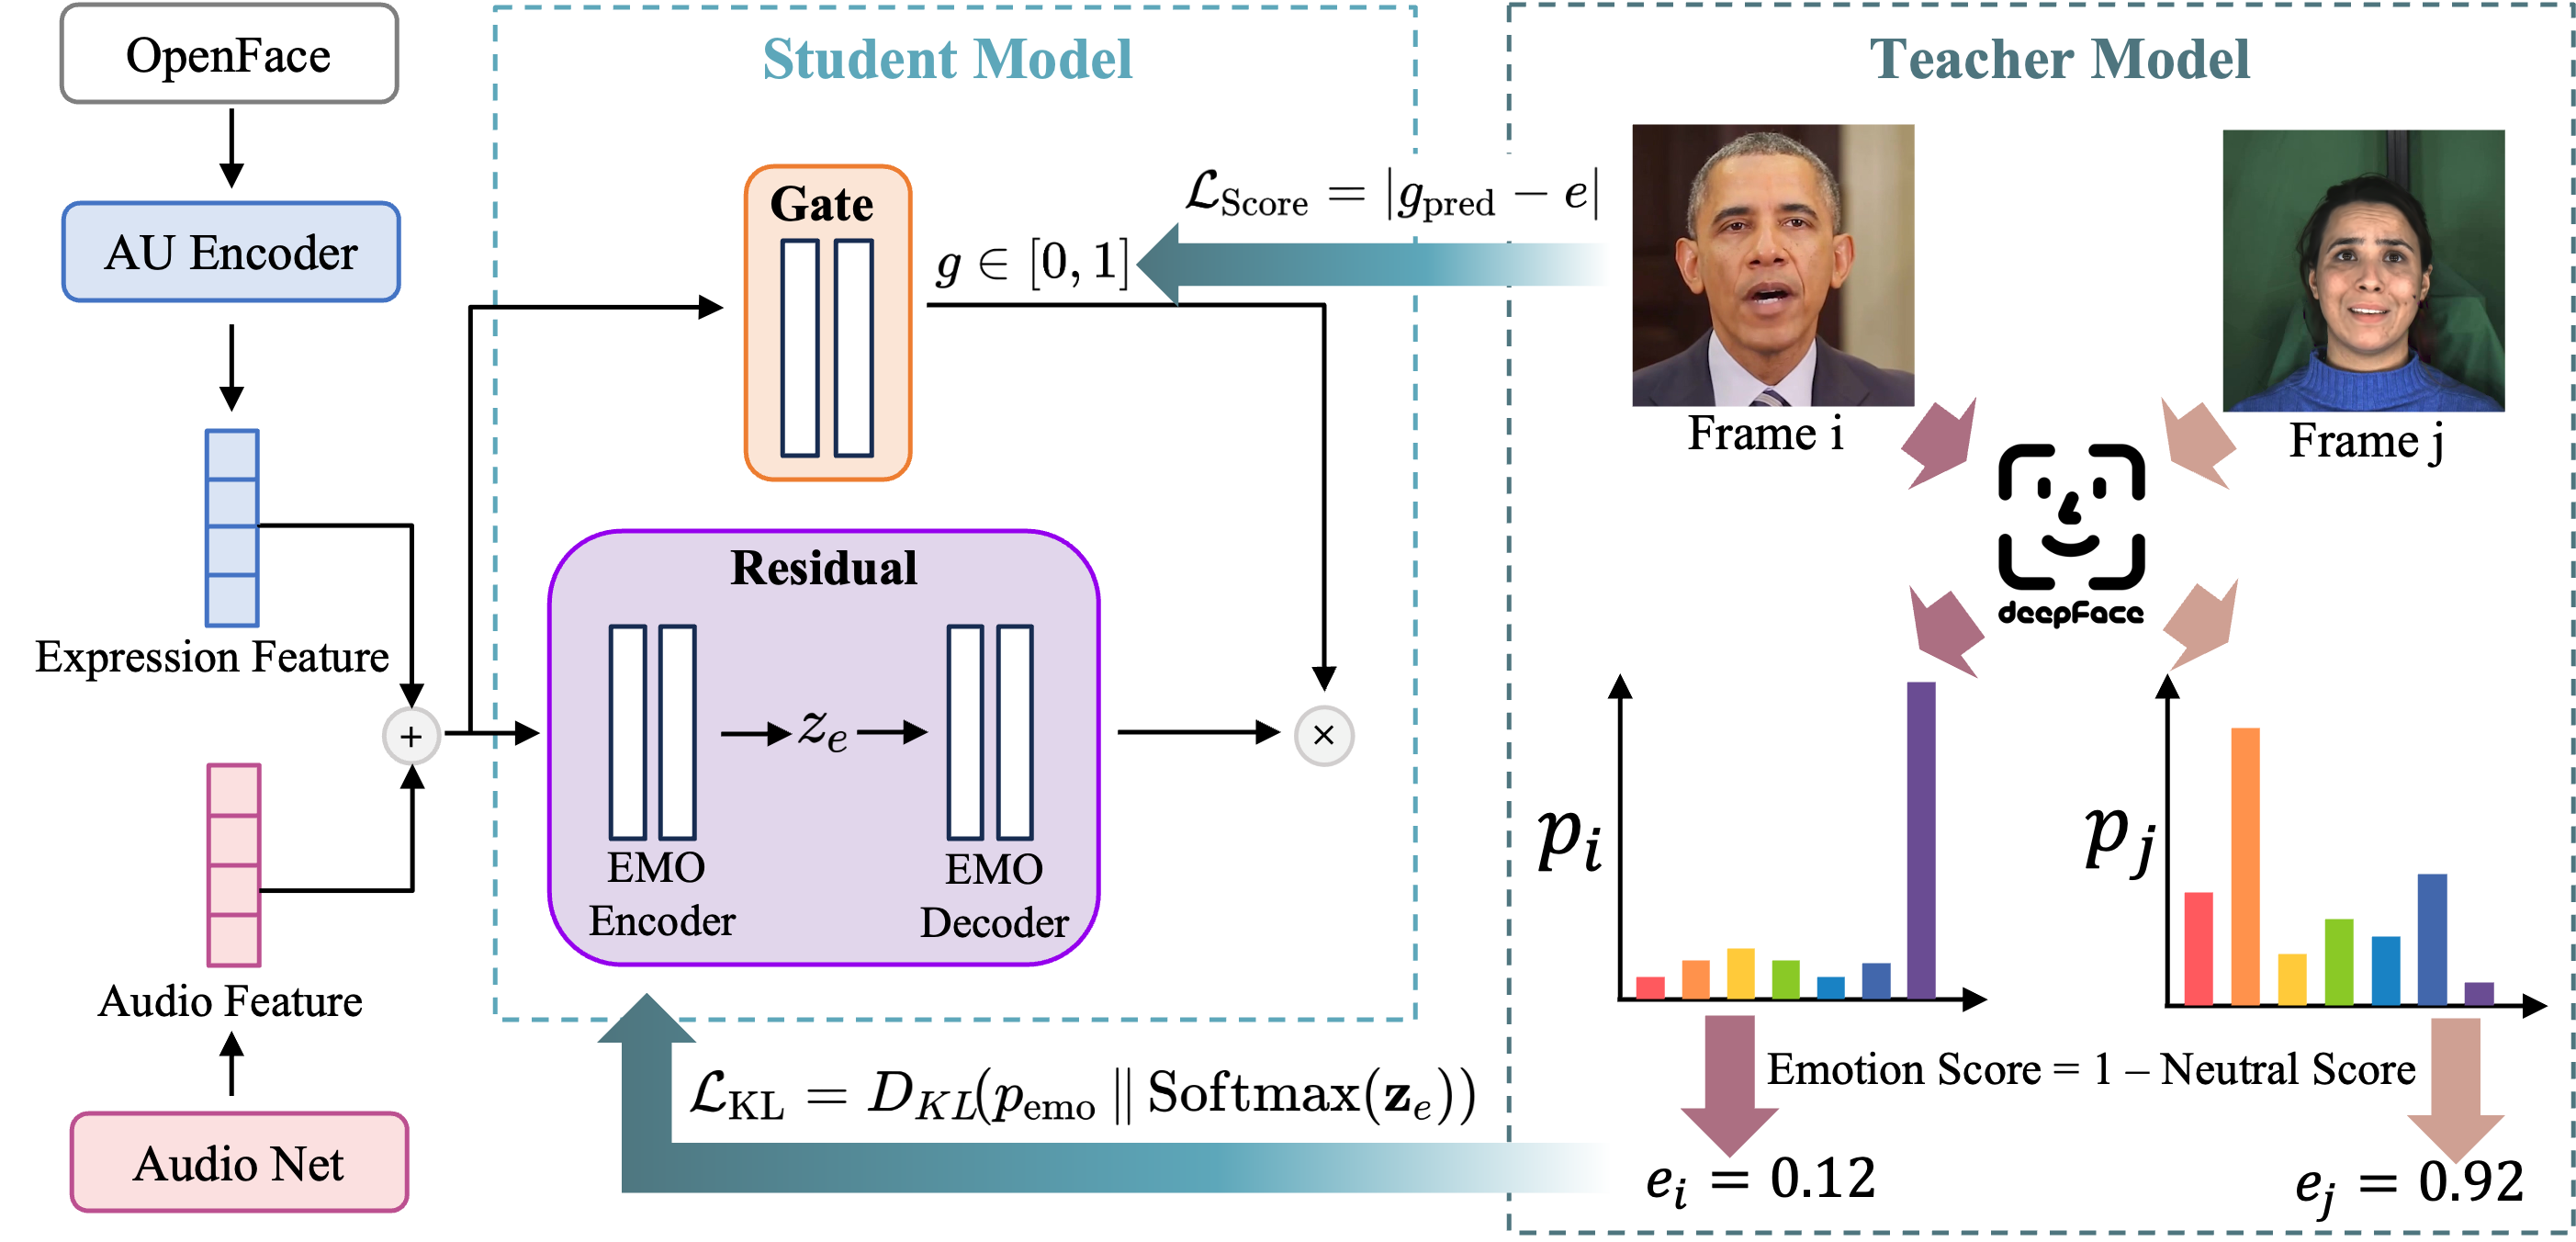
\includegraphics[width=\linewidth,trim={0 40 0 40},clip]{./Fig/SEG.pdf}
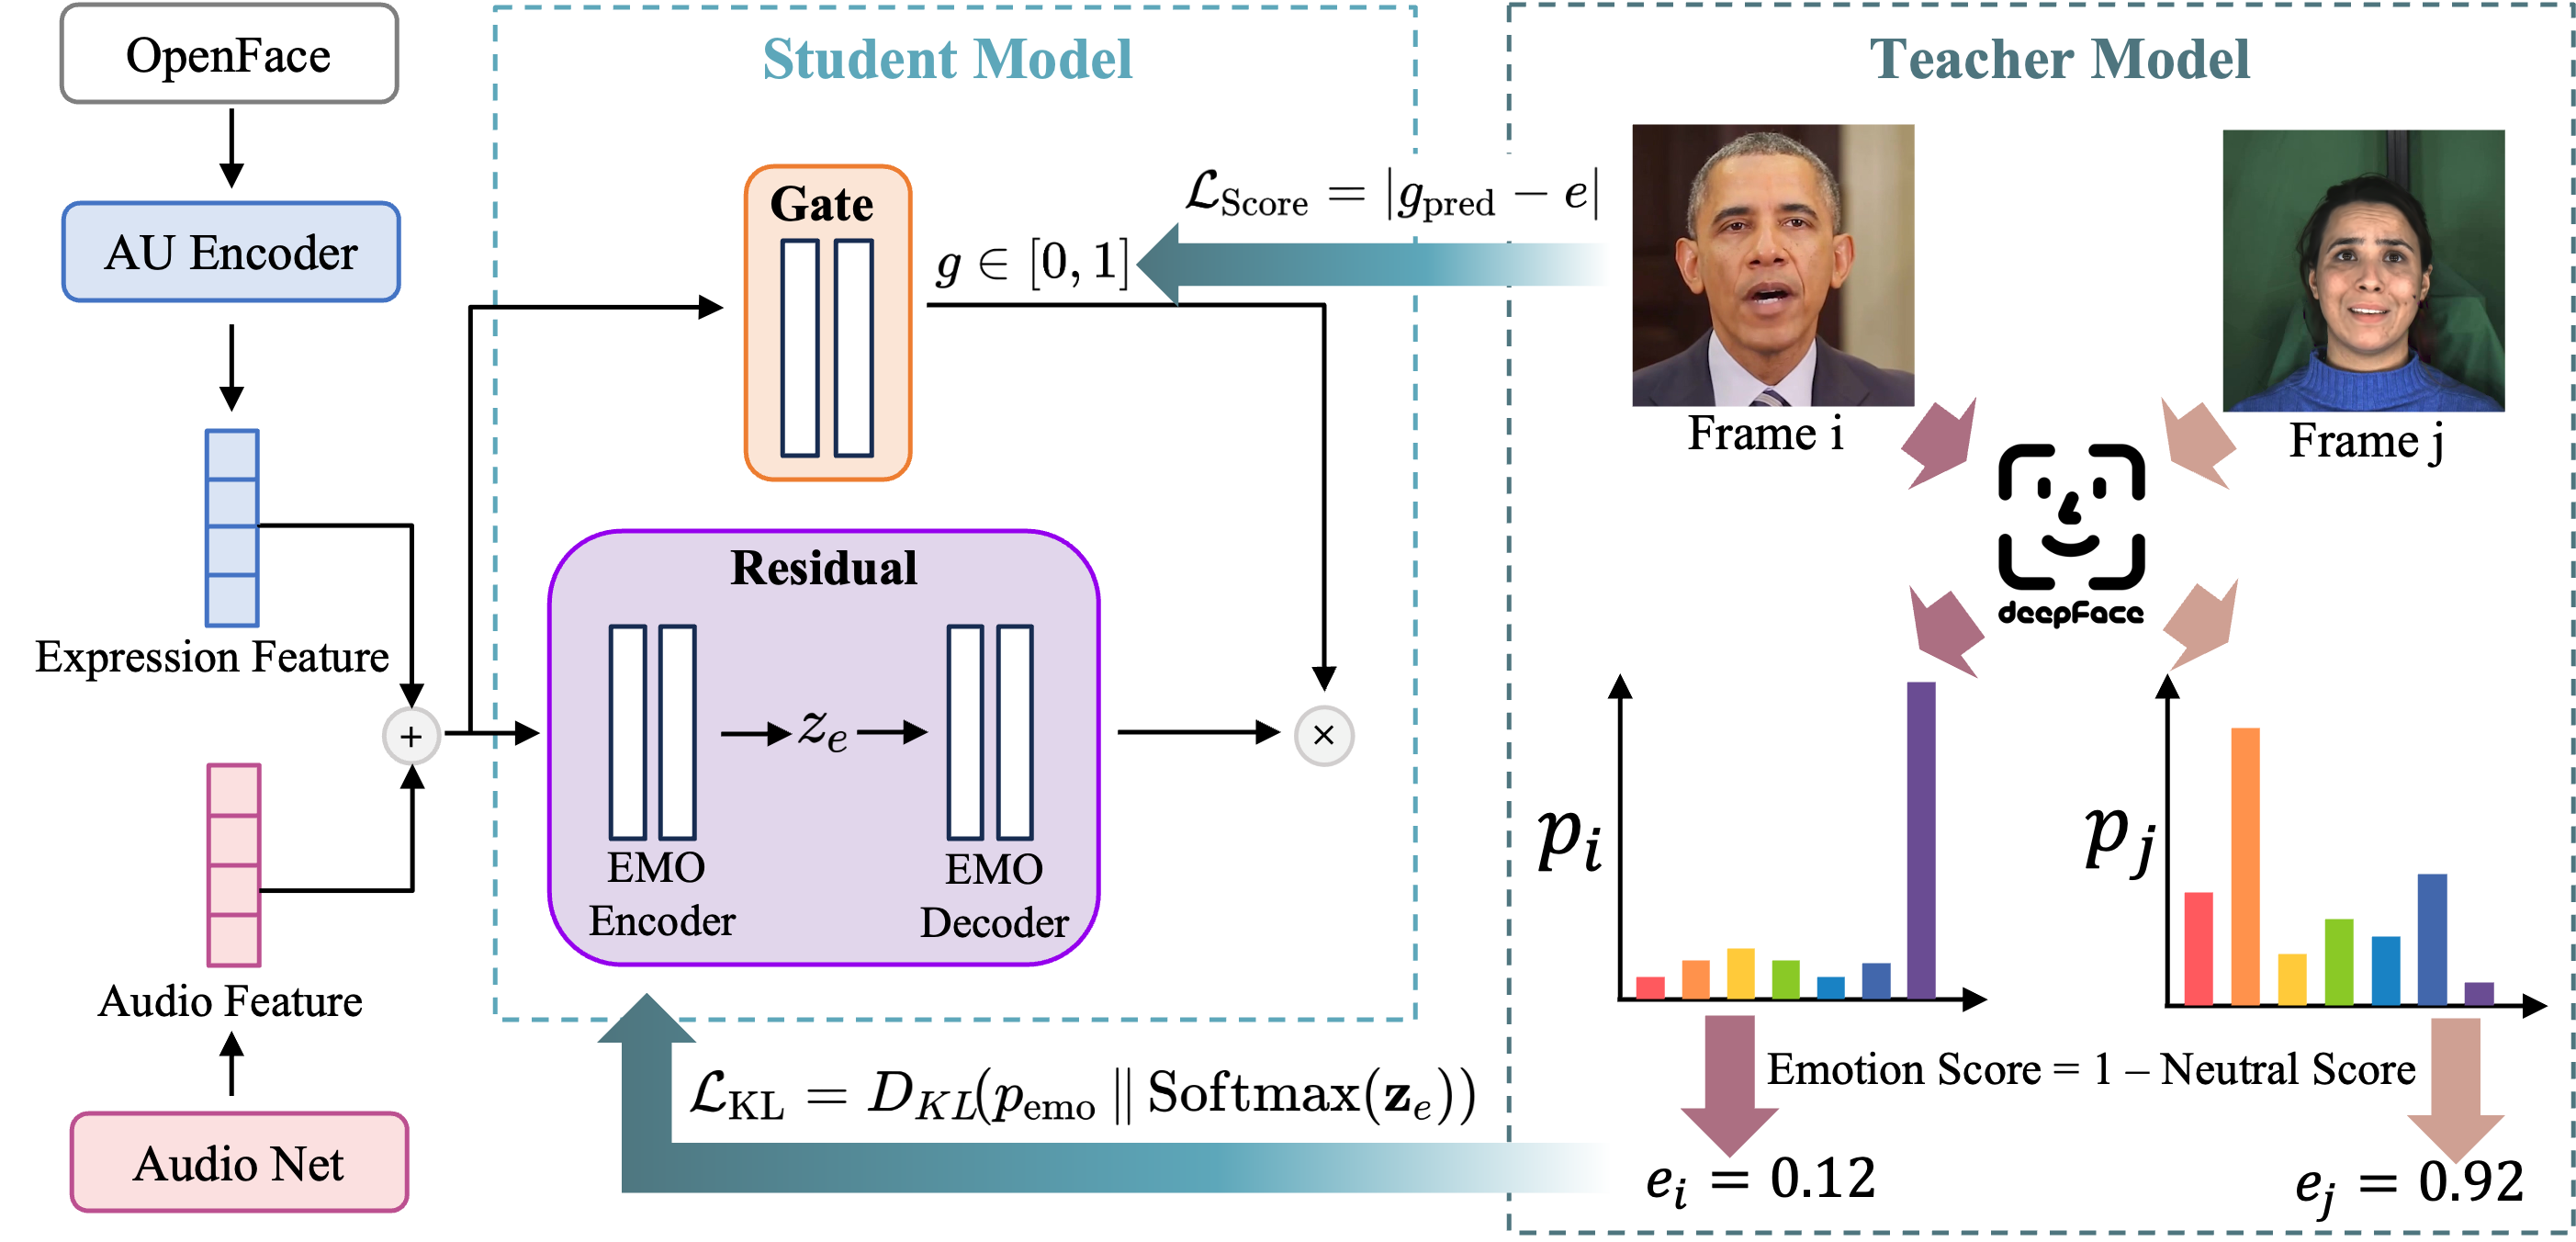
\includegraphics[width=\linewidth]{./Fig/SEG.png}
\vspace{-15pt}
\caption{ \textbf{Overview of Semantic Emotion Guidance.} DeepFace provides both a categorical emotion distribution and a scalar emotion score to guide GRMN’s residual and gate branches. } 
\vspace{-10pt}
\label{fig:seg} 
\end{figure}

\subsubsection{Semantic Emotion Guidance}
\label{sec:distill}
While GRMN supports structured motion decomposition, we incorporate explicit emotional supervision to enhance its sensitivity to emotion-driven variations. Given the scarcity and bias of manual annotations, we adopt a teacher-student distillation framework termed Semantic Emotion Guidance, as illustrated in Fig.~\ref{fig:seg}. An off-the-shelf emotion recognizer, DeepFace~\cite{serengil2024lightface}, serves as the teacher and provides two supervisory signals for each training frame:
(i) a normalized emotion distribution \(p_{\text{emo}}\) representing the probabilities of seven basic emotions, and 
(ii) a scalar emotion score \(e\) that measures the intensity of the current expression, defined as:
\begin{equation}
e = 1 - p_{\text{emo}}(\text{neutral}).
\label{eq:emotion-intensity}
\end{equation}

These teacher signals guide two submodules in GRMN: the residual branch captures emotion information by aligning its latent representation \(\mathbf{z}_e\) with the teacher’s emotion distribution \(p_{\text{emo}}\), while the gate branch learns emotion intensity by matching the scalar \(e\). This dual guidance enables GRMN to model both the type and intensity of emotions, yielding expressive yet controllable motion generation.



% Main result figure
\begin{figure*}[ht]
    \centering
    \includegraphics[width=1\textwidth]{./Fig/Qual_Results.png}
    \vspace{-10pt}
    \caption{
\textbf{Qualitative comparison on \textit{self-reconstruction}.} EmoTaG generates more expressive, temporally coherent, and well-synchronized talking heads than previous methods across both neutral and emotional test cases. It preserves accurate mouth articulation and natural upper-face motion even under challenging expressions. The red rectangles highlight regions where previous methods produce distorted and inaccurate facial motions. We strongly recommend watching the supplementary video for dynamic comparison.}
    \vspace{-10pt}
    \label{fig:Qual_Results}
\end{figure*}

\subsection{Pretrain \& Adaptation Framework}
During pretraining, the Gated Residual Motion Network (GRMN) learns a universal motion prior from a multi-identity corpus. During adaptation, we achieve efficient personalization by freezing the pretrained GRMN and only fine-tuning the AdaIN modulation parameters, which enables EmoTaG to capture identity-specific dynamics from just a 5-second video. Once the GRMN has been adapted, we perform inference using this personalized motion network. Because audio carries very limited information about upper-face expression or head pose, we additionally provide a set of pose \& expression frames as auxiliary inputs during inference, following the previous works~\cite{ye2024real3d,ye2024mimictalk,li2025instag}. These frames are processed by the FLAME Tracker to get head pose, and by the Expression Network to obtain upper-face cues. With new audio as the driving signal and the pose \& expression cues offering complementary conditioning, the adapted GRMN produces expressive and coherent facial motions that naturally correspond to the new audio.

\subsection{Training Objectives}

\label{sec:training}
Our full objective combines photometric, emotional, and geometric supervision:
\begin{equation}
\mathcal{L} = 
\mathcal{L}_{\text{Render}} +
\mathcal{L}_{\text{KL}} +
\mathcal{L}_{\text{Score}} +
\mathcal{L}_{\text{Geo}},
\end{equation}
where the first three losses are used in both pretraining and adaptation, while $\mathcal{L}_{\text{Geo}}$ is applied only during adaptation.

\noindent \textbf{Rendering loss.} 
Following 3D Gaussian Splatting~\cite{kerbl20233d}, the rendering loss ensures both pixel and structural fidelity:
\begin{equation}
\mathcal{L}_{\text{Render}} =
\mathcal{L}_{1}(I, I_{GT}) +
\lambda_{\text{D-SSIM}}\!\cdot\!(1 - \mathrm{SSIM}(I, I_{GT})),
\end{equation}
where $\mathcal{L}_{1}$ enforces color consistency, while SSIM~\cite{wang2004image} preserves perceptual structure.

\noindent \textbf{Emotion distillation losses.}  
To distill explicit emotion cues from the DeepFace~\cite{serengil2024lightface} teacher, the residual branch aligns its latent emotion representation $\mathbf{z}_e$ with the teacher-provided emotion distribution $p_{\text{emo}}$:
\begin{equation}
\mathcal{L}_{\text{KL}} = D_{KL}\!\left(p_{\text{emo}} \,\|\, \mathrm{Softmax}(\mathbf{z}_e)\right),
\end{equation}
while the gate branch regresses the teacher’s scalar emotion score $e$:
\begin{equation}
\mathcal{L}_{\text{Score}} = |g_{\text{pred}} - e|.
\end{equation}

\noindent \textbf{Geometric loss.}  
Following Gaussianpro~\cite{cheng2024gaussianpro}, we compute the 2D depth $D$ and normal $N$ maps from the rendered image $I$ during adaptation. These maps are compared against pseudo-ground-truths $D_{GT}$ and $N_{GT}$ from Sapiens~\cite{khirodkar2024sapiens}:
\begin{equation}
\mathcal{L}_{\text{Geo}} =
\mathcal{L}_{D}(D, D_{GT}) +
\mathcal{L}_{N}(N, N_{GT}).
\end{equation}
This auxiliary loss mitigates overfitting under limited visual supervision and preserves physically consistent facial geometry across frames.


% Main Table
\begin{table*}[t]
\centering
\small
\resizebox{\textwidth}{!}{
\setlength{\tabcolsep}{3pt}
\begin{tabular}{l|ccccccc|ccccccc|cc}
\toprule
\multirow{2}{*}{Method}
& \multicolumn{7}{c|}{\textbf{Neutral Set}} 
& \multicolumn{7}{c|}{\textbf{Emotional Set}} 
& \multicolumn{2}{c}{\textbf{Efficiency}} \\
\cline{2-17}
& PSNR$\uparrow$ & LPIPS$\downarrow$ & SSIM$\uparrow$
& LMD$\downarrow$ & \multicolumn{2}{c}{\rule{0pt}{2.4ex}AUE-(L/U)$\downarrow$} & Sync-C$\uparrow$
& PSNR$\uparrow$ & LPIPS$\downarrow$ & SSIM$\uparrow$
& LMD$\downarrow$ & \multicolumn{2}{c}{\rule{0pt}{2.4ex}AUE-(L/U)$\downarrow$} & Sync-C$\uparrow$
& Train$\downarrow$ & FPS$\uparrow$ \\
\midrule
Real3DPortrait~\cite{ye2024real3d}
& 25.41 & 0.053 & 0.827
& 3.415 & 1.143 & 1.084 & \cellcolor{bestblue}6.719
& 25.16 & 0.063 & 0.815
& 3.642 & 1.183 & 1.149 & \cellcolor{bestred}6.583
& -- & 8.9 \\
ER-NeRF~\cite{li2023efficient}
& 28.21 & 0.038 & 0.847
& 3.549 & 1.314 & 0.466 & 3.142
& 27.31 & 0.054 & 0.822
& 4.215 & 1.541 & 0.802 & 2.714
& 2 h & 33.2 \\
TalkingGaussian~\cite{li2024talkinggaussian}
& 28.43 & 0.034 & 0.844
& 3.582 & 1.167 & \cellcolor{secondblue}0.401 & 3.631
& \cellcolor{secondred}27.84 & 0.042 & 0.836
& 4.392 & 1.213 & \cellcolor{secondred}0.618 & 3.059
& 27 min & \cellcolor{bestred}118.4 \\
GeneFace++~\cite{ye2023geneface++}
& 27.58 & 0.044 & 0.835
& 3.521 & 1.212 & 0.647 & 3.737
& 27.16 & 0.047 & 0.824
& 3.721 & 1.253 & 0.961 & 3.588
& 7 h & 19.3 \\
MimicTalk~\cite{ye2024mimictalk}
& 25.26 & 0.071 & 0.857
& 3.478 & 0.964 & 0.781 & \cellcolor{secondblue}6.341
& 25.13 & 0.079 & 0.842
& 3.577 & \cellcolor{secondred}0.961 & 0.913 & 6.113
& 17 min & 8.6 \\
InsTaG~\cite{li2025instag}
& \cellcolor{secondblue}28.92 & \cellcolor{secondblue}0.029 & \cellcolor{secondblue}0.866
& \cellcolor{secondblue}3.145 & \cellcolor{secondblue}0.921 & 0.407 & 5.329
& 27.82 & \cellcolor{secondred}0.040 & \cellcolor{secondred}0.851
& \cellcolor{secondred}3.428 & 0.995 & 0.651 & 4.828
& \cellcolor{secondred}13 min & \cellcolor{secondred}82.5 \\
\textbf{EmoTaG (Ours)}
& \cellcolor{bestblue}30.02 & \cellcolor{bestblue}0.019 & \cellcolor{bestblue}0.883
& \cellcolor{bestblue}2.221 & \cellcolor{bestblue}0.685 & \cellcolor{bestblue}0.210 & 6.212
& \cellcolor{bestred}29.95 & \cellcolor{bestred}0.022 & \cellcolor{bestred}0.877
& \cellcolor{bestred}2.456 & \cellcolor{bestred}0.702 & \cellcolor{bestred}0.236 & \cellcolor{secondred}6.147
& \cellcolor{bestred}11 min & 76.4 \\
\bottomrule
\end{tabular}}
\vspace{-5pt}
\caption{\textbf{Quantitative comparison on \textit{self-reconstruction}} of neutral and emotional talking videos with 5s training data. \protect\bestbluebox{} and \protect\secondbluebox{} indicate the 1st and 2nd best results on the neutral set, while \protect\bestredbox{} and \protect\secondredbox{} indicate the 1st and 2nd best results on the emotional set. Efficiency columns (Train, FPS) are ranked using the red palette.}
\vspace{-10pt}
\label{tab:main}
\end{table*}

